\documentclass[12pt,twoside,a4paper]{report}
\usepackage{titlesec}       %To change the appearance of chapters/sections
\usepackage{titletoc}
\usepackage{setspace}%Enables commands: \singlespacing, \onehalfspacing
\usepackage{fancyhdr_mod}  %Defines proper headers suitable for a thesis
\usepackage{cardiff_thesis}   %Cardiff Thesis style
\usepackage[square,comma,numbers,sort&compress]{natbib}
\bibliographystyle{thesis}  %Thesis bibliography style
\parindent=20pt
\setcounter{section}{-1}

\usepackage{amsmath}
\usepackage{amssymb}

\usepackage{graphicx}% Include figure files
\newcommand{\mn}{_{\mu\nu}}
\newcommand{\fs}{\text{ .}}
\newtheorem{theorem}{Theorem}[section]
\newcommand{\pd}{\partial}
\newcommand{\infint}{\int^\infty_{-\infty} }
\newcommand{\Fp}{F^{+}_{\alpha}}
\newcommand{\Fx}{F^{\times}_{\alpha}}
\newcommand{\tbd}{\tilde{\textbf{d}}}
\newcommand{\tbh}{\tilde{\textbf{h}}}

\begin{document}
\title{Searching for Gravitational \\
         Waves}
\author{Iain Dorrington}
\supervisor{Patrick Sutton}
\supervisor{Stephen Fairhurst}
\firstreader{John Green}
\secondreader{John BigBooty}

\dedicate{
    This is the optional\\
    dedication page.\\
    Break lines up\\
    like this.
    }

\beforepreface

\prefacesection{Abstract}
An abstract is required in all theses.  Make sure that it fits
on one page!

\afterpreface



\chapter{Introduction}
\chapter{Gravitational Wave Astronomy in a Nutshell} 
\section{General Relativity}

Christoffel Symbol
\begin{equation} \label{christ}
\Gamma^\lambda\mn=\frac{1}{2}g^{\lambda \rho} [\partial_\nu g_{\mu \rho} + \partial_\mu g_{\nu \rho}-\partial_\rho g\mn]
\end{equation}
Riemann Curvature Tensor  
\begin{equation} \label{rct}
R^\mu_{\lambda \alpha \beta} = \partial_\alpha \Gamma^\mu_{\lambda \beta} -\partial_\beta \Gamma^\mu_{\lambda \alpha} + \Gamma^\mu_{\nu \alpha} \Gamma^\nu_{\lambda \beta} - \Gamma^\mu_{\nu \beta} \Gamma^\nu_{\lambda \alpha}
\end{equation}
Ricci Tensor
\begin{equation} \label{rt}
R\mn=g^{\alpha \beta} R_{\alpha \mu \beta \nu}=R^\beta_{\mu \beta \nu}
\end{equation}
Ricci Scalar
\begin{equation} \label{rs}
R=g^{\alpha \beta}R_{\alpha \beta}=R^\beta_\beta
\end{equation}
The Einstein Equations
\begin{equation} \label{eineq}
G\mn =R\mn -\frac{1}{2} R g\mn=\frac{8 \pi G}{c^4}T\mn
\end{equation}
Alternative form of the Einstein equations
\begin{equation} \label{alt einstein}
R\mn = \frac{8 \pi G}{c^4}\left( T\mn - \frac{1}{2}Tg\mn \right) 
\end{equation}


\section{Gravitational waves}
General Relativity shows that spacetime can curve and move. From this, it may seem obvious that waves can travel though spacetime. But this is not a trivial fact; Einstein himself, having introduced the concept of gravitational waves in 1916, later claimed they could not exist. In this section, we will show that gravitational waves do exist. We will do this by considering a perturbation of the flat Minkowski metric. We will then calculate the Ricci Tensor and Ricci Scalar for the perturbed metric and, with a clever choice of Gauge transformation, see that these yield a wave solution to Einstein's Equations. 

\subsection{Linearised Gravity}
Let $g\mn$ be the metric given by adding a small perturbation $h_{\mu\nu}$ to the Minkowski metric $\eta\mn=\text{diag}(-1,1,1,1)$. We write this metric as 
\begin{equation} \label{pert metric}
g\mn=\eta_{\mu\nu}+h_{\mu\nu} \text{, } \hspace{20pt} |h_{\mu\nu}| \ll 1 \text{ .}
\end{equation}

To first order in $h$, we calculate the Ricci tensor (\ref{rt})
\begin{equation} \label{lin rt}
R\mn =\eta^{\alpha \beta}R_{\alpha \mu \beta \nu} = \frac{1}{2}\left( \pd_\mu \pd ^\alpha h_{\alpha \nu} + \pd_\nu \pd_\alpha h^\alpha_\mu -\Box h\mn -\pd_\mu \pd_\nu h \right)
\end{equation}
and the Ricci scalar (\ref{rs}) 
\begin{equation} \label{lin rs}
R=\eta^{\mu \nu}R\mn=\pd _\mu \pd_ \alpha h^{\mu \alpha} - \Box h \textbf{,}
\end{equation}
where $\Box=\pd_\mu \pd^\mu $ is the d'Alembertian operator and $h=h^\mu_\mu$ is the trace of $h$. From these, we find the resulting Einstein tensor is also linear in $h$ 
\begin{equation} \label{lin Einstein}
G\mn =R\mn -\frac{1}{2} R g\mn \textbf{.}
\end{equation}

\subsection{Gauge Transformation}
With the following Gauge transformation, we can simplify the expression for the linear Einstein tensor
\begin{equation}
x^{\mu'}=x^\mu +\chi ^\mu (x)\text{,} \hspace{20pt}\chi \ll x\fs
\end{equation} 
As $\chi$ is small, we have $\partial_\mu \chi^\nu \ll 1$. This gives us
\begin{equation}
\frac{\pd x^\mu}{\pd x^{\alpha'}}=\delta^\mu_\alpha-\pd_\alpha\chi^\mu +\mathcal{O}(|\pd \chi|^2) \fs
\end{equation}  
Applying these results to our metric (\ref{pert metric}) we find
\begin{equation} 
g_{\alpha' \beta'}=\frac{\pd x^\mu}{\pd x^{\alpha'}}\frac{\pd x^\nu}{\pd x^{\beta'}}g\mn=g_{\alpha \beta}-\pd_\alpha \chi_\beta -\pd_\beta \chi_\alpha \fs
\end{equation}
Subtracting the Minkowski metric from each side, we find 
\begin{equation} \label{pert transf}
h_{\alpha' \beta'}=h_{\alpha \beta}-\pd_\alpha\chi_\beta-\pd_\beta\chi_\alpha \fs
\end{equation}

We have some freedom in choosing our $\chi$, so we impose the \textit{harmonic gauge condition}
\begin{equation} \label{harmonic gauge}
\partial_\mu h^\mu_\nu = \frac{1}{2} \partial_\nu h \text{,}
\end{equation}
where $h=h^\lambda_\lambda$. We can always choose a $\chi$ such that this is true. To see this, first note that $\partial'_\mu = \partial_\mu - (\partial_\mu \chi^\lambda) \partial_\lambda$. From this we find
\begin{equation}
(\partial_\mu' h_\nu^\mu - \frac{1}{2}\partial_\nu' h') \approx (\partial_\mu h^\mu_\nu - \frac{1}{2} \partial_\nu h ) -\partial^2 \chi_\nu \fs
\end{equation}
Thus, if we are given an $h$ such that \ref{harmonic gauge} is not true, we can choose a $\chi$ such that 
\begin{equation} \label{harmonic chi}
\partial^2 \chi_\nu = (\partial_\mu h^\mu_\nu - \frac{1}{2}\partial_\nu h) \fs
\end{equation}

Using \ref{harmonic gauge}, we can simplify the Ricci tensor and scalar
\begin{equation}
R\mn = -\frac{1}{2}\Box h\mn
\end{equation}
\begin{equation}
R=-\frac{1}{2}\Box h \fs
\end{equation}
Using these in the linearised Einstein equations (\ref{lin Einstein}) gives us
\begin{equation}
\Box h\mn - \frac{1}{2}\eta\mn\partial^2 h =-\frac{16\pi G}{c^4}T\mn \fs
\end{equation}
Alternatively, we can use \ref{alt einstein} to write this as
\begin{equation}
\Box h\mn = -16\pi G \left( T\mn -\frac{1}{2} \eta\mn T \right). 
\end{equation}
In a vacuum, the right hand side of this equation becomes zero, and we can recognise as the relativistic wave equation. 

\subsection{Physical Effects of Gravitational Waves}
The plane wave solution for the vacuum wave equation is
\begin{equation} \label{plane wave}
h\mn (x) = \epsilon\mn e^{ik_\alpha x^\alpha} 
\end{equation}
where $\epsilon\mn$, the polarisation tensor for the gravitational wave, is symmetric and constant, and $k^\alpha$ is the 4-wave-vector given by $k^\alpha = (\omega,\vec{k})$. Subsituting this into the vacuum wave equation, we find 
\begin{equation}
k^2 = -\omega^2 + \vec{k} =0 \fs
\end{equation}
Hence, gravitational waves travel at the speed of light. 

The polarisation tensor is not arbitrary: It must satisfy the wave equation and the harmonic gauge condition. Putting the wave solution \ref{plane wave} into the harmonic gauge condition \ref{harmonic gauge}, we find that gravitational waves are transverse
\begin{equation} \label{harmonic gauge2}
k^\mu \epsilon\mn = 0 \fs
\end{equation}
We can impose further gauge conditions as long as the harmonic gauge (and hence \ref{harmonic gauge2}) is not violated. As any transformation with $\partial^2 \chi = 0$ will satisfy \ref{harmonic chi}, and hence harmonic gauge condition, we express $\chi$ as 
\begin{equation} \label{chi form}
\chi_\nu = X_\nu e^{ikx} \fs
\end{equation}
Using \ref{chi form} and \ref{plane wave} in the transformation equation \ref{pert transf}, we find the transformation equation for the polarisation tensor
\begin{equation} \label{epsilon tranform}
\epsilon'\mn = \epsilon\mn -ik_\mu X_\nu - ik_\nu X_\mu \fs
\end{equation}
Taking the trace of this, we find
\begin{equation}
\epsilon'^\mu_\mu = \epsilon^\mu_\mu - 2ik^\mu X_\mu \fs
\end{equation}
Thus, we can impose the further gauge condition that the polarisation matrix be traceless by choosing coordinates such that $\epsilon^\mu_\mu = 2ik_\mu X^\mu$, and so fixing one element of $X^\mu$. We can fix the other elements of $X_\mu$ by setting $\epsilon_{i 0} = 0$ for $i=1,2,3$. We do this using \ref{epsilon tranform} to find
\begin{equation} \label{epsilon 0}
\epsilon'_{i 0} = \epsilon_{i 0} -ik_i X_0 - ik_0 X_i \fs
\end{equation}
Now we see that by setting $ \epsilon_{i 0} = ik_i X_0 - ik_0 X_i$, we have $\epsilon_{i 0} = 0$. As the polarisaton tensor is symmetric, we have $\epsilon^0_i=0$ as well.

These conditions give us that $\epsilon_{0 0} = 0$ as well. Using the fact that the polarisation matrix can be assumed traceless $\epsilon^\mu_\mu$, the wave solution \ref{plane wave} reduces the harmonic gauge condition \ref{harmonic gauge} to 
\begin{equation}
\partial_\mu h^\mu_\nu = 0 \fs
\end{equation}
As $\epsilon_{i 0} = 0$, in the $\nu = 0$ case, only the $\mu=0$ term is non-zero. Thus we are left with
\begin{equation}
\partial_\mu h^\mu_0 = \epsilon^0_0 i k_0 e^{ik_\alpha x^\alpha} = 0 \fs
\end{equation}
Which implies $\epsilon^0_0=0$. As the polarisaton tensor is symmetric, we have $\epsilon^3_3=0$ as well.  

We can make the polarisation tensor simpler by assuming the wave is traveling in the z-direction, that is $\vec{k} = (0,0,\omega)$. The transverse condition \ref{harmonic gauge2} then forces all the z-components of the polarisation matrix to be zero, $\epsilon^3_i = \epsilon^i_3 = 0$. The wave solution \ref{plane wave} now looks like
\[
h\mn (x)
=
\begin{bmatrix}
0 & 0 & 0 & 0 \\
0 & a & b & 0 \\
0 & b & -a & 0 \\
0 & 0 & 0 & 0 
\end{bmatrix}
e^{(i\omega (z-t))} \fs
\] 

\newpage
\section{Gravitational Waves Sources} 
\begin{itemize}
\item GW generation 
\item Sources
\begin{itemize}
\item BBH - Multiple found already
\item BNS - One found and Hulse-Taylor
\item NSBH
\item GRB 
\item SN
\item Unknown
\end{itemize}
\end{itemize}
\section{How to Detect Gravitational Waves} 
Can cite soaulson and the noises paper
\begin{itemize}
\item Michelson Interferometer (cite R.Weiss 1972 paper to look smart)
\item Measure change in output power due to interference in the arms
\item Noise sources and how they are mitigated
\begin{itemize}
\item Fundamental noise
\item Environmental noise
\item Instrumental noise
\item Noise budget
\end{itemize}
\end{itemize}
\subsection{How to find something interesting in all that noise}
\begin{itemize}
\item Autocorrelation function
\item PSD and ASD (tie back to the noise budget) 
\item Matched filtering (for 1 detector)
\item Unmodelled search (for 1 detector)
\item Network statistics (coincident and coherent) 
\end{itemize}

\chapter{The Compact Binary Coalescence Search} \label{CBC search}
\section{PyCBC overview}
\begin{itemize}
\item Overview of pipeline based on technical paper
\item Consistency checks
\item The O2 search (coincident)
\end{itemize}
\section{PyGRB}
\begin{itemize}
\item Has sky position 
\item Coherent
\end{itemize}


\section{O2 PyGRB Search} 

\section{The O3 PyCBC search}
\begin{itemize}
\item More detectors strengthens the case for coherent search
\item Hierarchical search, using coincident search to find location 
\end{itemize}

\chapter{Undmodelled Search}
\section{Xpipeline}
\section{Subthreshold GRBs}

\chapter{Machine Learning for GW Astronomy}
\section{\label{intro}Introduction}
% LIGO and virgo operate a network of ifos, looking for GWs. Detected BBH and BNS. Other sources have unknown WF morphology due to poorly understood physics of the sources. Hence, we need unmodelled searches. 
The Laser Interferometer Gravitational Wave Observatory (LIGO) and Virgo collaborations operate ground-based Gravitational Wave (GW) detectors. They have detected signals of astrophysical origin, including the merger of a Binary Neutron Star (BNS) system and multiple Binary Black Hole (BBH) merger signals. As these sources have a known signal morphology, they can be found using a highly sensitive matched-filter search, as discussed in chapter \ref{CBC search}. But some of the most interesting possible sources, such as core collapse supernova, do not have a known waveform morphology. For this reason, it is important to develop unmodelled searches as well. 

% Current searches apply thresholds on a small number of detection statistics such as SNR, chi2, or the cross-correlation between detectors. MVA can use the full dimensionality of the parameter space. 
In unmodelled searches we look for coherence between the data streams of multiple interferometers. We will consider the case of a Burst search where the sky position of the candidate source is known. This allows us to calculate the relative time of arrival in each detector and the relative signal power in each detector as well. 

%We begin by producing multiple coherent time series from the interferometer network data. We then identify times of excess coherent energy, which we call \textit{triggers}. A number of statistics are then calculated to measure the coherence of each trigger. We apply thresholds to the coherent energies to reduce the number of triggers, and then rank the remaining triggers. These thresholds are often applied to a some combination of a small number of the coherent energies calculated. By using \textit{Multivariate Analysis} (MVA) we can make cuts that use the whole parameter space.  

In this chapter, we will first discuss how an existing targeted Burst search, called \textit{X-pipeline}, searches for Gravitational Wave Bursts (GWBs). We will then see how we can improve this pipeline by using \textit{Multivariate Analysis} (MVA) to apply cuts and rank triggers.  

% The analysis starts with a list of triggers of known classification (signal or background) and properties. BG events are glitches from data, signal events are injections added to real ifo data. Each trigger is randomly assigned to either the signal or training set. The signal set are then used to train a classifier, i.e. learn where in the parameter space corresponds to signal triggers or BG triggers. We then test the classifier on tesitng set. 


\section{\label{xtriggers}Xpipeline}
Xpipeline is a data analysis pipeline for the Burst search. It begins by using the known sky location of the GRB to time-shift the data from each detector so that the GW arrives simultaneously in each data stream. Xpipeline then makes coherent data-streams from the individual detector data. There are two types of coherent data-streams: \textit{signal streams}, which increase the power of a GW signals, and \textit{null streams}, which reduce the power of true GW signals but not noise. \textit{Triggers} are groups of neighbouring pixels that are above threshold in a time-frequency map of a signal stream (see fig.\ref{fig:tfmap}). Xpipeline then removes triggers based on cuts of the various network data streams (see fig.\ref{fig:xcuts}). The position of these cuts is set to give the best performance on a subset of the triggers that are used for tuning. For the MVA pipeline, the position of these cuts is instead set by a machine learning algorithm (as we will see in \ref{ML}).

\begin{figure} % Example of including images
\begin{center}
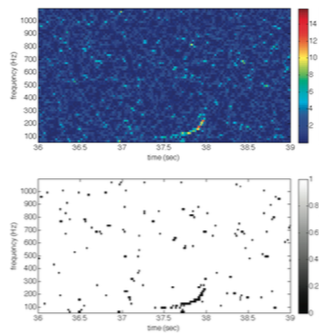
\includegraphics[width=0.8\linewidth]{xpipelineTFmap.png}
\end{center}
\caption{\textbf{Xpipeline Time-Frequency Map} This figure shows a time-frequency map from Xpipeline for a $1.4-10M_\odot$ NSBH merger. The top figure shows the $E_+$ energy and the bottom figure shows the top 1\% of pixels. } %\cite{xpipeline_paper}
\label{fig:tfmap}
\end{figure}

\begin{figure} % Example of including images
\begin{center}
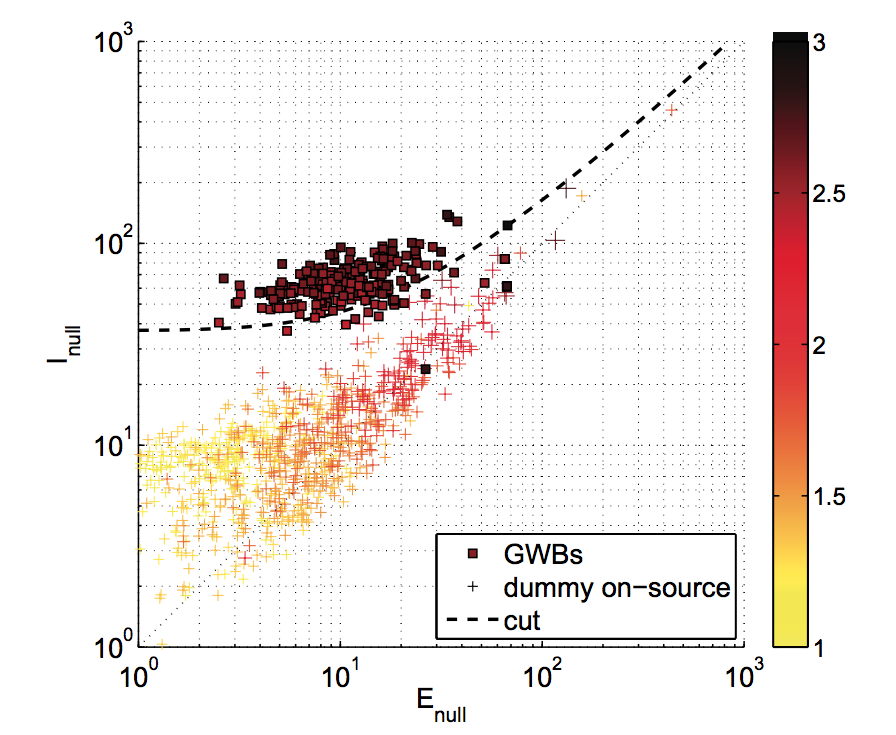
\includegraphics[width=0.8\linewidth]{xpipeline_cut.png}
\end{center}
\caption{\textbf{Xpipeline Cut} This figure shows Xpipeline making a cut to eliminate many spurious signals. } %\cite{xpipeline_paper}
\label{fig:xcuts}
\end{figure}

In this section, we will formulate two of the coherent data-streams generated by Xpipeline, as illustrative examples. The first is a signal-stream, called the \textit{standard likelihood}. We will then use the standard likelihood to create a null-stream. 

\subsection{Burst Search Background}
Suppose we have a network of $D$ detectors. A gravitational wave, described by $h_+(t)$ and $h_\times (t)$, passes through the Earth from direction $\hat{\Omega}$. We describe the sensitivity of detector $\alpha \in \{1,...,D \}$ to the plus and cross polarizations using the \emph{Antenna Response Functions}, denoted $\Fp (\hat{\Omega})$ and $\Fx(\hat{\Omega})$. The position of detector $\alpha$ is denoted by $\textbf{r}_\alpha$ and the noise in this detector is given by $n_\alpha (t)$. The detector output $d_\alpha (t)$ is then given by
\begin{equation} \label{det_output}
d_\alpha (t + \Delta t_\alpha (\hat{\Omega})) = \Fp (\hat{\Omega}) h_+ (t) + \Fx (\hat{\Omega}) h_\times (t) + n_\alpha (t + \Delta t_\alpha (\hat{\Omega})) \fs
\end{equation}   
Here $\Delta t_\alpha$ is the time taken for the GW to reach the detector from some arbitrary reference point\footnote{The center of the Earth is a fairly intuitive choice for a worldwide detector network.} $\textbf{r}_0$

\begin{equation}
\Delta t_\alpha (\hat{\Omega})=\frac{1}{c}(\textbf{r}_0-\textbf{r}_\alpha)\cdot\hat{\Omega} \fs
\end{equation}
%To understand why this time delay only appears in the noise of the above equation, think of the GW passing through the point $\textbf{r}_0$ at time $t$. The antenna response functions and the GWs waveform will not change between $\textbf{r}_0$ and $\textbf{r}_\alpha$, so the first two terms in \ref{det_output} are fixed. But it will take $\Delta t_\alpha$ to reach the detector, and so we must consider the noise in the detector at that moment to correctly determine the detectors output. 
From now on we will suppress explicit mention of the reference point $\textbf{r}_0$ or the time delay $\Delta t_\alpha$ on the understanding that detector outputs need to be time-shifted by an appropriate amount. 

In reality, detector outputs are not continuous but sampled discretely. The discrete Fourier transform $\tilde{x}[k]$ of the time series $x[j]$, and its inverse, are given by
\begin{equation}
\tilde{x}[k]=\sum^{N-1}_{j=0} x[j] e^{-i 2\pi jk/N}, \hspace{20pt}x[i]=\frac{1}{N}\sum^{N-1}_{j=0} \tilde{x}[k] e^{i2 \pi jk/N} \fs
\end{equation}
For sampling rate is $f_s$ and $N$ data points in the time domain, we convert continuous to discrete notation by using
\begin{equation}
x(t)\rightarrow x[j]
\end{equation} 
\begin{equation}
\tilde{x}(f)\rightarrow f^{-1} \tilde{x}[k]
\end{equation} 
\begin{equation}
\int dt \rightarrow f_s^{-1}\sum_j
\end{equation} 
\begin{equation}
\int df \rightarrow f_s N^{-1} \sum_k
\end{equation} 
\begin{equation}
\delta(t-t')\rightarrow f_s \delta_{jj'}
\end{equation}
\begin{equation}
\delta(f-f')\rightarrow N f_s^{-1}\delta_{kk'} \fs
\end{equation}  
For example, the one-sided noise spectral density for a detector with noise $n(t)$ can be written in continuous form as
\begin{equation}
\langle  \tilde{n}^* (f) \tilde{n} (f') \rangle = \delta (f-f') \frac{1}{2} S_n (f)
\end{equation}
where the angle brackets indicate an average over the noise. In the discrete notation listed above, this becomes
\begin{equation}
\langle  \tilde{n}^*_\alpha [k] \tilde{n}_\beta [k']  \rangle = \frac{N}{2} \delta _{\alpha \beta} \delta _{k k'} S_\alpha [k] \fs
\end{equation}
We will be working with the \emph{noise-spectrum-weighted} quantities, defined by
\begin{equation}
\tilde{d}_{w\alpha}[k]=\frac{\tilde{d}_\alpha [k]}{\sqrt{\frac{N}{2}S_\alpha [k]}}
\end{equation}
\begin{equation}
\tilde{n}_{w\alpha}[k]=\frac{\tilde{n}_\alpha [k]}{\sqrt{\frac{N}{2}S_\alpha [k]}}
\end{equation}
\begin{equation}
F^{+,\times}_{w\alpha}(\hat{\Omega},k)=\frac{F^{+,\times}_\alpha (\hat{\Omega})}{\sqrt{\frac{N}{2}S_\alpha [k]}}
\end{equation}
The normalisation of the whitened data is 
\begin{equation}
\langle  \tilde{n}^*_\alpha [k] \tilde{n}_\beta [k']  \rangle = \delta _{\alpha \beta} \delta _{k k'}  \fs
\end{equation}
In vector notation, we can write \ref{det_output} as
\begin{equation}
\tilde{\textbf{d}}=\textbf{F}\tilde{\textbf{h}}+\tilde{\textbf{n}} 
\end{equation}
where $\textbf{F}=[\textbf{F}^+ \:\:\:\textbf{F}^\times]$ and $\tilde{\textbf{h}}=[\tilde{h}_+ \:\:\: \tilde{h}_\times]^T$.

\subsection{Standard Likelihood}
Assume that the noise in our detectors is Gaussian. As a gravitational wave $\tilde{\textbf{h}}$ passes through the detector from a known direction, the probability of attaining whitened detector output $\tilde{\textbf{d}}$ in one time-frequency pixel is given by
\begin{equation}
P(\tilde{\textbf{d}}|\tilde{\textbf{h}})=\frac{1}{(2\pi )^{D/2}}\exp \left[ -\frac{1}{2} \left| \tbd - \textbf{F} \tbh  \right|^2 \right] \fs
\end{equation}  
For a set $\{ \tbd \}$ of $N_p$ time-frequency pixels, we have
\begin{equation}
P(\{ \tilde{\textbf{d}} \}|\{ \tilde{\textbf{h}} \})=\frac{1}{(2\pi )^{N_p D/2}}\exp \left[- \frac{1}{2} \sum_k \left| \tbd [k] - \textbf{F}[k] \tbh [k]  \right|^2 \right] \fs
\end{equation}  
By comparing this value to the probability that the detector produces this output in the absence of any GW signal, we can calculate a likelihood of the signal being a real GW signal. 

The \emph{Likelihood Ratio} $L$ is the log of the probability that the detector network will have output $ \tilde{\textbf{d}}$ in the presence of GW $\tbh$  divided by the probability of obtaining the same output in the absence of a gravitational wave ($\tbh=0$)
\begin{equation}
L=\ln \frac{P(\{ \tilde{\textbf{d}} \}|\{ \tilde{\textbf{h}} \})}{P(\{ \tilde{\textbf{d}} \}|\{ 0  \})}= \frac{1}{2} \sum_k \left[ \left| \tbd  \right|^2 - \left| \tbd - \textbf{F} \tbh   \right|^2  \right] \fs
\end{equation}

For the above analysis to be applied, we would need to know the waveform $\tbh$ in advance. For GRBs and other unmodelled searches, this is not possible. One way to handle this problem is to fit the waveform in each time-frequency pixel to the data in such a way as to maximise the likelihood ratio. Hence we have
\begin{equation}
0=\frac{\partial L}{\partial \tbh} \bigg|_{\tbh=\tbh_{\textbf{max}}} \fs
\end{equation} 
Solving this, we find
\begin{equation} 
\tbh_\textbf{max}=(\textbf{F}^\dagger \textbf{F} )^{-1} \textbf{F}^\dagger \tbd
\end{equation}
where the superscript dagger $^\dagger$ denotes the conjugate transpose. 

Calculating the likelihood ratio for $\tbh_\textbf{max}$ gives us the \emph{Standard Likelihood} $E_\text{SL}$
\begin{equation} \label{Esl}
E_\text{SL}=2L(\tbh_\textbf{max} )=\sum_k \tbd^\dagger \textbf{P}^\text{GW} \tbd
\end{equation}
where 
\begin{equation} \label{projOp1}
\textbf{P}^\text{GW} \equiv \textbf{F} (\textbf{F}^\dagger \textbf{F})^{-1} \textbf{F}^\dagger \fs
\end{equation}
We can see from equation \ref{det_output} that the contribution made to the data output by a passing GW from fixed sky location is restricted to the subspace spanned by $\textbf{F}_+$ and $\textbf{F}_\times$. Therefore the energy in this subspace is the energy that is consistent with a GW from a given sky location. We can show that $\textbf{P}^\text{GW} $ is a projection operator, projecting the data into this same subspace. The standard likelihood maximises the energy in this subspace, and so is the maximum energy contained in the whitened data that is consistent with a GW from the given sky location.\footnote{In practice, some of this energy will be due to noise. We say that the energy due to noise is \emph{inconsistent} with a GW signal. The rest of the energy must be due to the GW, so we say it is \emph{consistent} with the GW.} This is an example of the coherent signal-streams that Xpipeline uses.
\subsection{Null Energy}
We can use the standard likelihood to find a null-stream. First consider the \emph{total energy}, given by
\begin{equation}
E_\text{tot}=\sum_k | \tbd |^2 \fs
\end{equation}
This is an incoherent statistic as it contains only auto-correlation terms, and no cross-correlation terms. If we subtract the standard likelihood from the total energy, we obtain the \emph{null energy}
\begin{equation} \label{Enull}
E_\text{null} \equiv E_\text{tot}-E_\text{SL}=\sum_k \tbd ^\dagger \textbf{P}^\text{null} \tbd \fs
\end{equation}
This is the energy that is inconsistent with a GW from given sky location, and must therefore be associated with noise. This is the minimum amount of energy in our whitened data that is inconsistent with our GW. It is an example null-stream used by Xpipeline.

This shows one of the key advantages of coherent analysis. If we analysed our data incoherently, we would be working with just the total energy. But using coherent methods, we can project the whitened data into the subspace spanned by $\textbf{F}^+$ and $\textbf{F}^\times$, thus removing some fraction of the noise without removing any of the signal. The drawback is that if the sky position is not known in advance, then the analysis needs to be repeated for a set of directions that span the entire sky ($\gtrsim 10^3$ directions), each with different antenna response functions $\textbf{F}^+$ and $\textbf{F}^\times$. This will slow down analysis and increase the false alarm probability.

\subsection{Incoherent Energy and Background Rejection}
The diagonal elements of \ref{Enull} are auto-correlation terms, and the other elements are cross-correlation terms. The auto-correlation part of the null energy are called the \textit{incoherent energy}, and denoted by
\begin{equation}
I_\text{null} = \sum_k \sum_\alpha P^\text{null}_{\alpha \alpha} | \tilde{d}_\alpha |^2 \fs
\end{equation}
Background triggers are typically not correlated between the different detectors of the network, so the cross-correlation terms are small relative to the auto-correlation terms. This means that for glitches, we have
\begin{equation} \label{glitch energy}
E_\text{null} \approx I_\text{null} \fs
\end{equation} 
Compare this to the case of a GW signal. This will be correlated between the detectors. By construction, the energy of the correlated energy does not appear in the null-stream. Therefore, in the presence of a strong GW, the incoherent energy is much larger than the null energy 
\begin{equation} \label{GW energy}
E_\text{null} \ll I_\text{null} \fs
\end{equation}
Using \ref{glitch energy} and \ref{GW energy}, we see that the ratio of $E_\text{null}$ and $I_\text{null}$ is very different in the case of a glitch as opposed to a GW signal. We can use this to make the following cut to remove noise triggers from our sample
\begin{equation} \label{cut}
I_\text{null} / E_\text{null} > C
\end{equation}
for some constant $C>1$. This test does not work as well for small amplitude glitches, where the statistical fluctuations can lead to $E_\text{null}$ being smaller than $I_\text{null}$. For this reason, Xpipeline varies $C$ with the size of the trigger. The precise position of the cut is set to maximise performance on a set of injections.  
 
\section{\label{ML}Machine Learning}
We have seen how Xpipeline makes cuts on coherent statistics to distinguish between noise and GW signals. You can see from \ref{cut} that the cut only uses two statistics, the null energy and the incoherent energy. Xpipeline generates many coherent statistics that could used in conjunction to make a more powerful cut. In this section we discuss how to use Machine Learning to make achieve this. The software we use is the Toolkit for Multivariate Analysis package in the ROOT data analysis framework. 

\subsection{Supervised Machine Learning}
The type of Machine learning we use is called \textit{supervised machine learning}. Supervised machine learning algorithms are trained on data which has already been classified. They can then be shown a new, not-classified data point and determine the appropriate classification. Supervised machine learning requires data to be in a particular format (see table \ref{table:1}). It is a list of \emph{events}, each with a \emph{label} and corresponding \emph{attributes}. The machine learning algorithm builds a \textit{classifier} that can determine the label of an event when given the event's attributes. In the case of our GW search, the events are the triggers returned by Xpipeline (see section \ref{xtriggers}). The labels are \textit{signal} or \textit{background}, and the attributes are the values of the signal and null data streams for those triggers as well as some statistics describing the trigger, e.g. peak frequency, trigger duration. The signal triggers are generated by injecting signal waveforms into the data. Background triggers are triggers that do not coincide with an injected signal.

%As explained in the introduction, in this paper we look at two machine learning classifiers. The details of these classifiers are described in sections \ref{bdt} and \ref{mlp}. In this section we give some background on machine learning. 

The signal and background trigger sets are each divided into two subsets: The \emph{training set} and the \emph{testing set}. The training set is used to build the classifier, while the testing set is used to measure the accuracy of the trained classifier. If the classifier performs much better on the training set than on the testing set, then the classifier is \emph{overtrained}. This means that the classifier has learned exactly the properties of signals and noise in the training set, rather than learning the general properties of signals and noise. When an overtrained classifier is used on a different data set with different noise properties (such as the testing set), it will perform poorly. 

\begin{table}
\begin{tabular}{| c | c | c | c | c |} 
 \hline
Label & loghbayesiancirc & standard & circenergy & circinc  \\ [0.5ex] 
 \hline\hline
Background & 12.3128 & 58.3523 & 44.7196 & 24.9015 \\ 
 \hline
Background & 12.0349 & 67.5344 & 41.7045 & 22.4848 \\
 \hline
Signal & 18.2145 & 59.8136 & 53.3320 & 22.0601 \\
 \hline
Signal & 43.7113 & 123.9194 & 118.9774 & 43.9234 \\
 \hline
Signal & 6422.1467 & 14426.9124 & 14167.2933 & 4991.7876 \\ [1ex] 
 \hline
 
\end{tabular}
\caption{An example of MVA training data. Each event has a label and several attributes.}
\label{table:1}
\end{table}


\subsection{Boosted Decision Trees} \label{bdt}
A \textit{Decision Tree} is a simple type of classifier. It is a flowchart of true/false statements about a trigger's attributes to determine the correct label. For example, consider the decision tree shown in fig.\ref{fig:tree}. Here the attributes are labeled as the components of a vector $x$. We start at the top node and work downwards. If the node is true then we follow the branch to the left and if not then we follow the branch to the right. We then consider the statement at the end of whichever branch we follow. We continue this process until we reach a \textit{leaf node}, which has no branches and contains a final classification for the trigger.  
\begin{figure} % Example of including images
\begin{center}
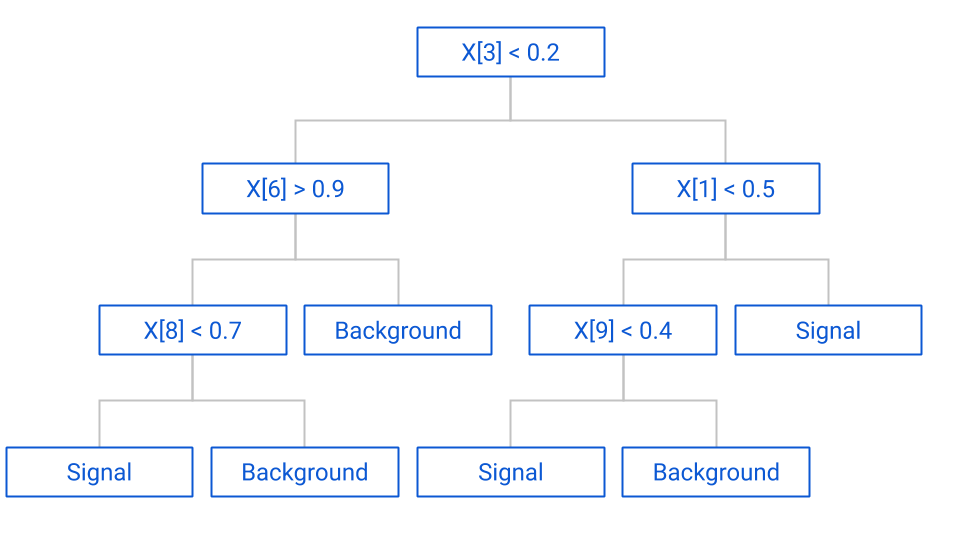
\includegraphics[width=0.8\linewidth]{Decision_tree.png}
\end{center}
\caption{\textbf{A decision tree example} To determine if a trigger is a signal or noise event the tree makes a series of cuts on the attributes x[N]. If the inequality in a node is true, then the next node is the branch to the left. Otherwise the next node is the one to the right. }
\label{fig:tree}
\end{figure}

We can improve the performance of the classifier by using an \textit{ensemble} (or \textit{forest}) of trees. This means training multiple distinct trees, and each tree independently classifies the trigger. The final classification of each trigger is a normalised sum of the outputs of each tree, with +1 corresponding to signal, and -1 corresponding to background. This leads to different regions of the parameter space having different MVA scores, as can be seen in fig.\ref{fig:mvacuts}. The higher the score, the more likely an event is to be a signal. 

\begin{figure} % Example of including images
\begin{center}
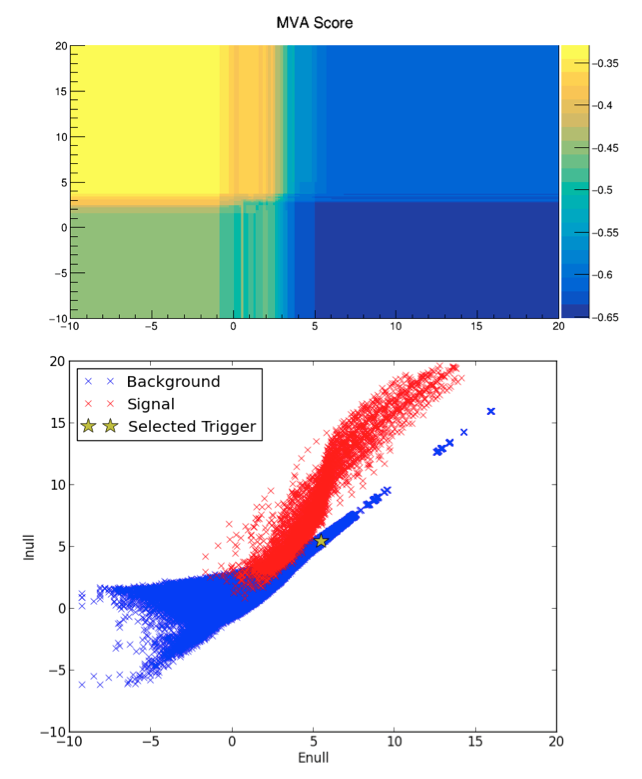
\includegraphics[width=0.8\linewidth]{mva_trigger_and_score.png}
\end{center}
\caption{\textbf{Visualising the Classifier} In the bottom plot you can see the value for log(Enull) and log(Inull) for all the signal and background training data used to build the classifier. We chose one of these events at random (indicated by the star) and varied Enull and Inull to see how it changed the MVA score, indicated by the colour in the top plot. As you can see, increasing Inull and decreasing Enull leads to the event being more likely to be classed as a signal. This is akin to the xpipeline cut shown in fig.\ref{fig:xcuts}. }
\label{fig:mvacuts}
\end{figure}


To train a decision tree, we need methods to find the variable to cut on and the position of the cut for each decision node, and the label in each leaf node that best discerns between signal and background. Each of these values is set by brute force: Trying each possible combination of cuts and labels to get the best performance on the training events. Ensemble methods work best when each classifier in the ensemble is independent of the others, so training every tree on the same events is not going to give optimal results. For this reason each tree is trained on some subset of the training set.  We could pick events at random to form these subsets, but a more powerful method is to use \textit{Adaptive Boosting}. 

When using adaptive boosting, each event in the training set is given a probability that it will be selected to train the next tree. Initially each event in the training set has the same probability of being selected. Then after each tree is trained the probability of each event being selected to train the next tree is updated such that misclassified events are more likely to be included in the training set for the next tree. The misclassifed events have their probability of being selected for training the next tree updated by the \textit{boost weight}, given by
\begin{equation}
\alpha = \frac{1 - \text{err}}{\text{err}} 
\end{equation}
where err is the misclassification rate. The weights are then renormalised. 

Note that the boost weight is greater than one for\footnote{The misclassification rate is always less than half when the labels only take two possible values as the algorithms we use are always better than chance alone.} err$< 1/2$, and that as the error gets smaller, the boost weight increases. The effect of this is that each new tree is more likely to be trained on the events that are most difficult to classify. 

The ensemble output is also changed, so that it is weighted rather than being a simple sum. If the output of the $i$th tree is given by $h_i(\textbf{x})$, with $\textbf{x}$ being the event attributes, then the ensemble output is given by
\begin{equation}
H(\textbf{x}) = \frac{1}{N}\sum_{i=0}^N \ln(\alpha_i)h_i(\textbf{x)}
\end{equation}  
where $N$ is the number of tree in the ensemble. Small values indicate background events, while large values indicate a signal. 

\subsection{Data Preprocessing}\label{data-preprocessing}
Extra data preprocessing is required for the training set. Suppose a small amplitude signal injection is added close to a large amplitude glitch in the data. This trigger will be labeled as a signal, due to the injection, but the properties of the trigger will resemble a glitch, as the glitch has a much larger amplitude than the signal injection. It is essentially a background trigger labeled as a signal. This has two affects: It reduces our ability to detect real signals by making the properties of signals harder for the algorithm to learn, and it can lead to background triggers being misclassified as a Gravitational Wave signal.  

For these reasons, it is important to make sure that signal injections do not overlap in time or frequency with background triggers. To prevent this from happening we \textit{clean} the data. This means finding all of the triggers in the data for the smallest signal injection scale. The injected waveforms are too small to be detected so all of these triggers must be background. We then increase the injection amplitude and look for triggers again. Any triggers that overlap in time or frequency with the noise triggers are then identified and removed from the from the signal set. \textbf{This description of cleaning may need to change if we change the cleaning codes.}

We must also not include injections in our signal set that are too small to be detected. If we do then we would again be including triggers labeled as signal that have the properties of a noise trigger, even if there is no glitch present. For this reason we apply a threshold on the amplitude of the signal set, so any injection below that amplitude is removed. The level of the threshold is set experimentally; If it is too low then we will increase the chance of a false positive and hurt our sensitivity to real signals, but if it is too high then we will limit the classifiers ability to detect low amplitude signals. 

We also use \textit{Generalised Clustering}. This is a change in the way Xpipeline defines a trigger. Without using generalised clustering, triggers are groups of neighbouring pixels in the time-frequency maps such as in fig.\ref{fig:tfmap}. Generalised clustering allows these pixels to be separated by a user-specified number of pixels. This can boost the signal power of long triggers, as long triggers tend to contain breaks in their time-frequency maps that causes Xpipeline to list a single long trigger as multiple short triggers. The downside to using generalised clustering is that it can cause noise triggers to be grouped together as well, boosting the power of noise. This then causes our sensitivity to short triggers to be reduced slightly. Experimenting with generalised clustering in both the standard Xpipeline analysis and the MVA analysis suggests that the benefits outweigh the costs, with an improvement of between 7\% and 50\% for long inspiral and adi waveforms at the cost of a decrease of 3\% to 9\% for short sine-gaussian waveforms.  

As XTMVA is to be used for the unmodelled search, it is also important to ensure that the search can find waveforms that are not in the training set. There are several tools that we use to achieve this. The first is to limit the amount of information the classifier is given about the waveform morphology. The classifier cannot know the precise morphology of any waveform because the only attributes that the classifier trains on is the time, peak-frequency, and various measurements of the coherent and null energy between the detectors in the network. This forces the classifier to use the coherence of the triggers to make a classification, rather than the waveform morphology. 

There is still a possibility that the classifier will become too specialised to the waveforms in the training set, as the classifier is given peak frequency data and certain waveform morphologies may have particular characteristics than become apparent from the coherent and null streams. For this reason we also trained the classifier on a variety of different waveforms. The training set included long and short waveforms, and a variety of different morphologies. Some of the signals are astrophysically motivated, such as compact binary coalescence signals, while some are artificial, such as the white noise burst.

The final tool we use to ensure the classifier is sensitive to generic waveforms is to test the classifier on waveforms that are not included in the training set. If the classifier can find waveforms not in the training set, then we can be reasonably confident that it is sensitive to generic waveforms. We also try removing certain waveforms from the training set to test the robustness of the classifier. This will lead to a drop in sensitivity for that waveform, but if the drop in sensitivity is small, then we can be confident that the classifier is robust. 

\subsection{Optimisation and Validation} \label{opt}
With any machine learning algorithm, there are \textit{hyperparameters} that must be tuned. The number of trees in the ensemble, the maximum depth of the trees, and many more hyperparameters must be chosen. We optimise the hyperparamters by repeatedly running an example analysis with different hyperparameters, trying to increase the number of injected signals we could recover from the testing set. 

Setting our hyperparameters using the testing set can cause \textit{data leakage}. Data leakage is when data from outside the training set is used to build a classifier. As we tune our classifier on the testing set, it is possible that we will implicitly tune our classifier to only work well on this training and testing set. This is very similar to overtraining discussed in section \ref{ML}. To avoid this, once we have tuned the hyperparameters on a single GRB, we test the classifier on several other GRBs. If the performance drops significantly on these other GRB analyses, then we have had data leakage and we need to retune our classifier. This process of testing on previously unused data is called \textit{validation}. If there is evidence of data leakage, then we must retune our classifier and validate it again, this time using a different (previously unused) GRB so as to avoid data leakage from the validation GRB. 

Optimisation is a somewhat cyclical process, as once we have changed one hyperparameter, we must then go back and test that other parameters do not now need changing. But optimisation is not pure guess work, and in the rest of this section we will see the strategy we used to optimise our classifier. We first discuss optimising the training data to use. As mentioned in section \ref{data-preprocessing}, there are several choices to make regarding what data is used for training, such as setting the amplitude threshold. We then discuss optimising the BDT classifier itself. 

\subsubsection{Training Set}
Many of the hyperparameters mentioned in section \ref{data-preprocessing} had to be optimised. Consider the amplitude threshold applied to triggers before they are included in the training set. If this is too low then noise triggers contaminate the signal training set, but if it is too high then we limit the sensitivity of our classifier to only higher amplitude waveforms. 

We also optimised the waveforms that are included in the training set, whether to use cleaning or not, and whether to use generalised clustering. \textbf{Write more on this once we've done it.}



\begin{itemize}
\item Had to optimise the threshold as well
\item Training waveforms
\item cleaning or not
\item Gen clustering or not
\end{itemize}

\subsubsection{BDT Parameters}
There are many hyperparameters that need to be set for a BDT analysis. In this section we discuss some of these hyparameters and the method we used to optimise them for our analysis. 

We began by setting values for \textit{NTrees}, the number of trees in the ensemble, and the learning rate, discussed in section \ref{bdt}. These two parameters are set first to ensure the machine learning algorithm will converge in a reasonable amount of time. Setting the learning rate  too low causes the classifier to take longer to converge. Setting the learning rate too high can cause the classifier to never converge. Similarly, using too many trees takes too long for the classifier to finish training, but too few and the training will terminate before the algorithm has converged. Setting these first ensures that we have a classifier that gives sensible results in a reasonable amount of time. While optimising, we set these values slightly high, to ensure that our classifier converges and does so quickly while we optimise our other parameters. Once the other parameters are set, we again optimise NTrees and the learning rate, increasing the number of trees and decreasing the learning rate to ensure the algorithm reaches its optimum performance, even if it increases the time taken for training.

We now tune the tree-specific parameters. Unlike the number of trees and the learning rate which are primarily tuned to ensure the classifier will converge in a reasonable time, these parameters are set to ensure that the classifier is accurate but does not overtrain. Overtraining can happen when the trees are allowed to make cuts that are too fine, carving out regions of parameter-space around anomalous events in the training set rather than finding cuts that generalise beyond the training data. The way to prevent this is to limit how fine the cuts made by the decision trees are allowed to be, while allowing cuts that are fine enough to pick out the general features of signal and background events in our data. There are several hyperparameters we can set to do this, which must all be tuned. 

The first of these is the maximum depth of the trees, which is the maximum number of cuts a tree can make before it reaches a leaf node. Each cut divides the parameter-space into ever smaller regions which it labels as background or signal. Setting the maximum number of cuts too low will therefore cause the classifier to be too coarse in dividing up the parameter-space, resulting in poor accuracy. Increasing the maximum depth allows the classifier to pick out smaller features in the parameter-space. If the maximum depth is too high then the classifier will overtrain; dividing the parameter-space into precisely the regions that work for the training set and losing generality. As we are using adaptive boosting, it is recommended \textbf{cite TMVA userguide} to use trees with fewer cuts. For this reason we tried values from 2-16, finding that for our problem a maximum depth of 8 was optimal. 

A related hyperparameter is the minimum number of events that we allow in a leaf node. If we allow the training algorithm to have any number of events in a leaf node, then it will occasionally find cuts that results in a small number of events in one or more of the leaf nodes. The again allows for the carving out of anomalous events in the training set rather than finding cuts that can generalise beyond the training set. Conversely, setting the minimum number of events allowed in the leaf nodes to be too high does not allow the classifier to pick out the key features in the data. We used a grid search over the values 100-1600 for the minimum number of events per leaf node and found the optimal value to be 400. 

The final hyperparameter we set is the number of cuts that the training algorithm scans over to find the best cut. When the classifier is training it searches for the best way to cut the parameter-space into a signal subspace and a background subspace. To do this we can try every possible cut on every parameter. This can be very slow and lead to overtraining. To speed up our analysis and reduce the chance of overtraining, we can choose the number of cuts to try on each parameter. For example, we may decide to use 10 cuts for each parameter. In this case the algorithm will tune the cut on a parameter which ranges from 0-100 by trying cuts at 0,10,20,... and selecting the best of these cuts. To tune the number of cuts we wanted to use, we tried values from 10-160 as well as allowing the classifier to try every possible cut. We found that 80 cuts was optimal for our purposes. 

\begin{itemize}
\item This can definitely be phrased better
\end{itemize}

\subsubsection{Result of Optimisation}
\begin{itemize}
\item Show nice plots of improved sensitivity due to optimisation
\item Show improvement when compared to Xpipeline
\end{itemize}


\end{document}
